\documentclass[a4paper,12pt]{article}
\usepackage{graphicx}
\usepackage[margin=0.3in]{geometry}

% Default fixed font does not support bold face
\DeclareFixedFont{\ttb}{T1}{txtt}{bx}{n}{12} % for bold
\DeclareFixedFont{\ttm}{T1}{txtt}{m}{n}{12}  % for normal

% Custom colors
\usepackage{color}
\definecolor{deepblue}{rgb}{0,0,0.5}
\definecolor{deepred}{rgb}{0.6,0,0}
\definecolor{deepgreen}{rgb}{0,0.5,0}
\definecolor{green}{rgb}{0,0.8,0}

% Python style for highlighting
\usepackage{listings}
\newcommand\pythonstyle{\lstset{
language=Python,
basicstyle=\ttm,
otherkeywords={self},             % Add keywords here
keywordstyle=\ttb\color{deepblue},
emph={MyClass,__init__},          % Custom highlighting
emphstyle=\ttb\color{deepred},    % Custom highlighting style
stringstyle=\color{deepgreen},
commentstyle=\color{green},
frame=tb,                         % Any extra options here
showstringspaces=false            % 
}}

% Python environment
\lstnewenvironment{python}[1][]
{
\pythonstyle
\lstset{#1}
}
{}

% Python for external files
\newcommand\pythonexternal[2][]{{
\pythonstyle
\lstinputlisting[#1]{#2}}}

% Python for inline
\newcommand\pythoninline[1]{{\pythonstyle\lstinline!#1!}}

\begin{document}

\section{Random Walk}
%\lstinputlisting[language=Python]{../random_walk.py}
\pythonexternal{../random_walk.py}
The above code took 6.3 seconds to run.

For the most part, the residuals fall within error bars as expected. The two sets of error bars are close, but the Poisson error bars (red) are consistently larger than those from the histogram variance (green).

\begin{figure}[h]
    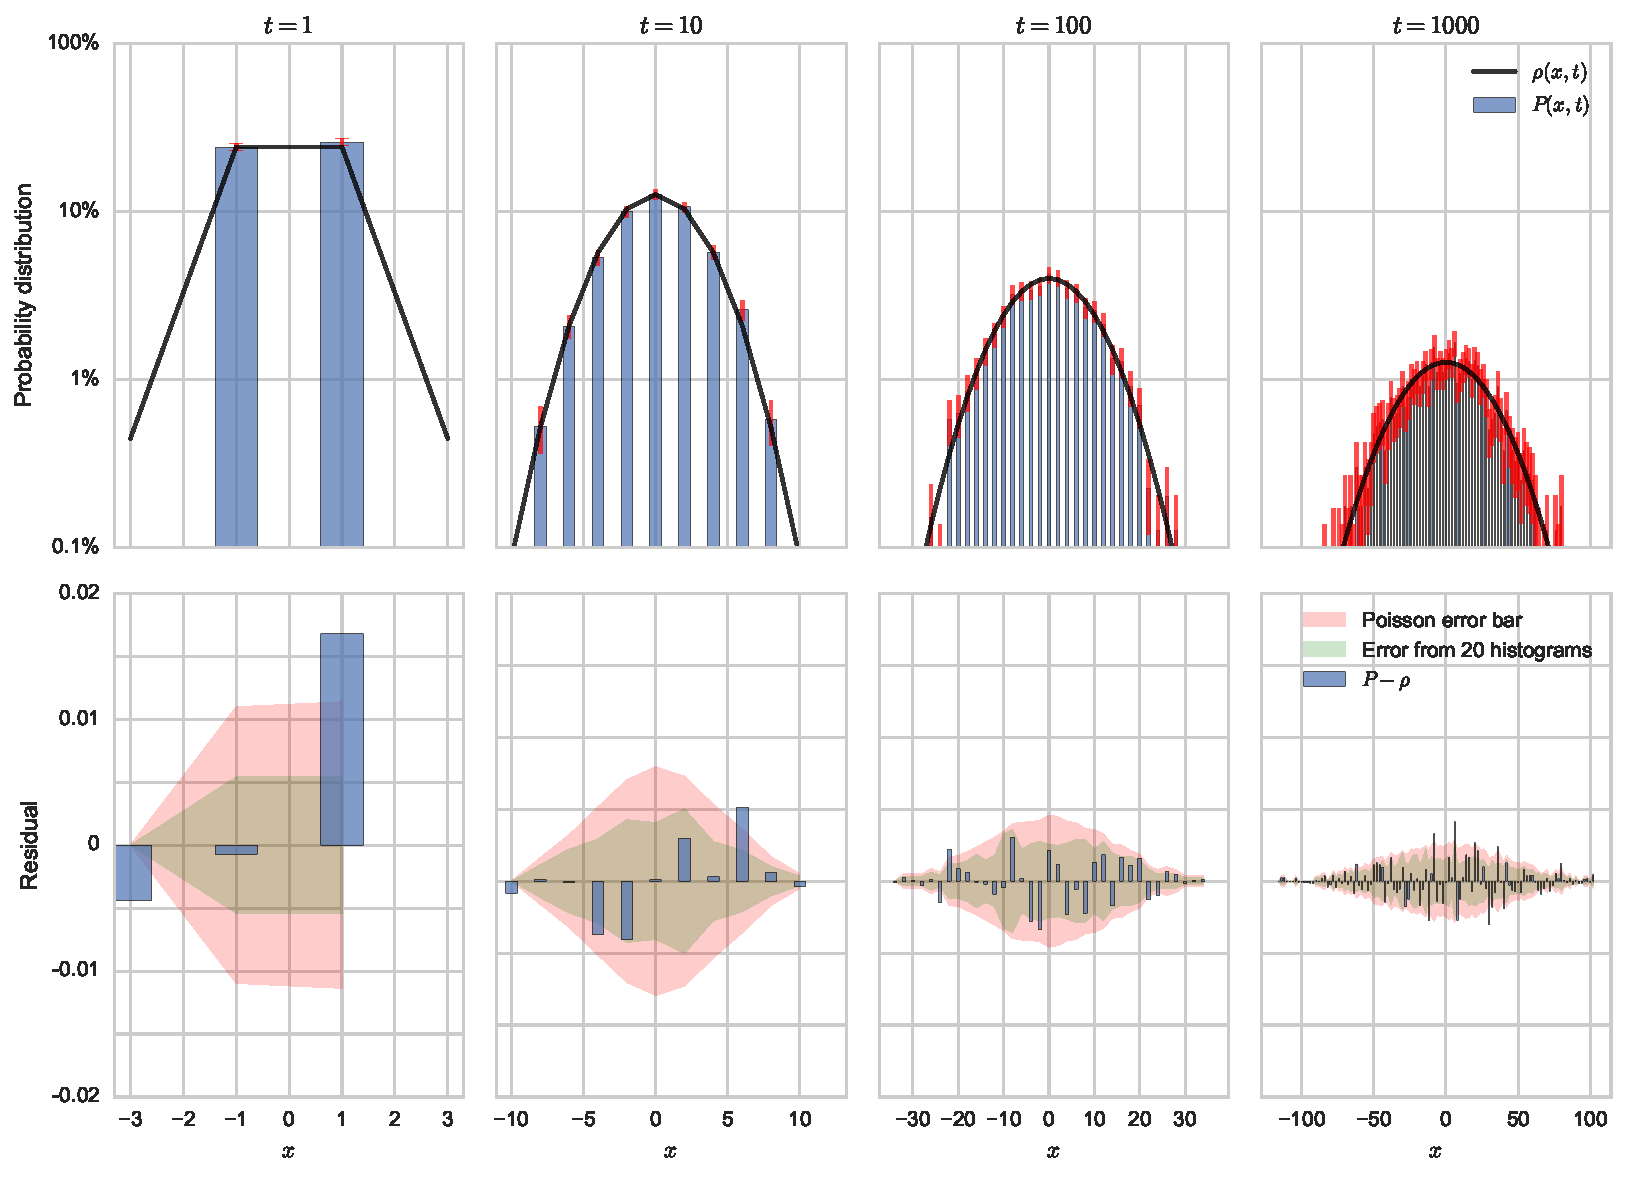
\includegraphics[width=\linewidth]{../random_walk.pdf}
\end{figure}

\newpage

\section{Self-avoiding Random Walk}
\pythonexternal{../saw.py}
This program ran for approximately 10 hours to complete $N = 1e8$ random walks,
but recorded no walks at times longer than $2^7$ (128) steps. The counts per
step were as follows:

\begin{tabular}{l | r}
    $t$ & random walks \\
    \hline
    1 & 100000000 \\
    2 & 100000000\\
    4 & 92594705\\
    8 & 67620778\\
    16 & 30042667\\
    32 & 4816814\\
    64 & 99311\\
    128 & 34\\
    256 & 0\\
\end{tabular}

As expected, the scaling of $R \sim L^\nu$ was different from a simple random walk with
$\nu = 0.5$. From the best fit, the data scales as $\nu = 0.735$, close to the given
theoretical value $\nu = 0.75$.

\begin{figure}[h]
    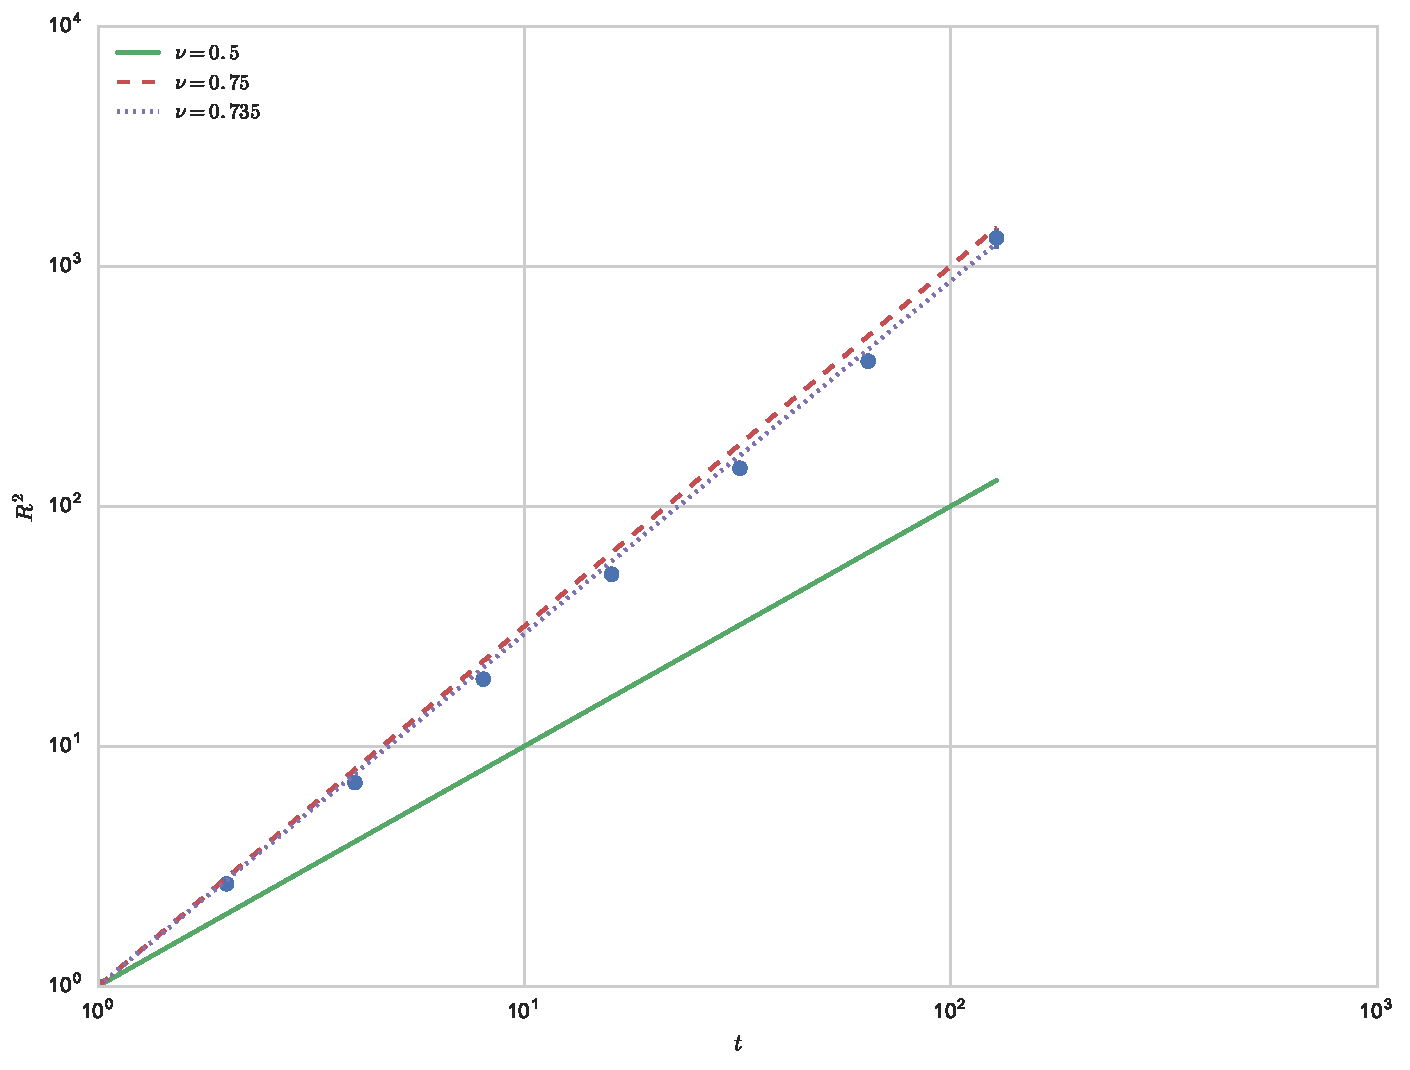
\includegraphics[width=0.9\linewidth]{../saw.pdf}
\end{figure}

\end{document}
